\begin{problema}
	Resolver:
\begin{enumerate}
	\item Localice en un plano los puntos $A(1,1)$, $B(3,4)$, $C(-2,5)$ y $D(-3,2)$. 
	\begin{sol}.
		\begin{figure}[H]
			\centering
			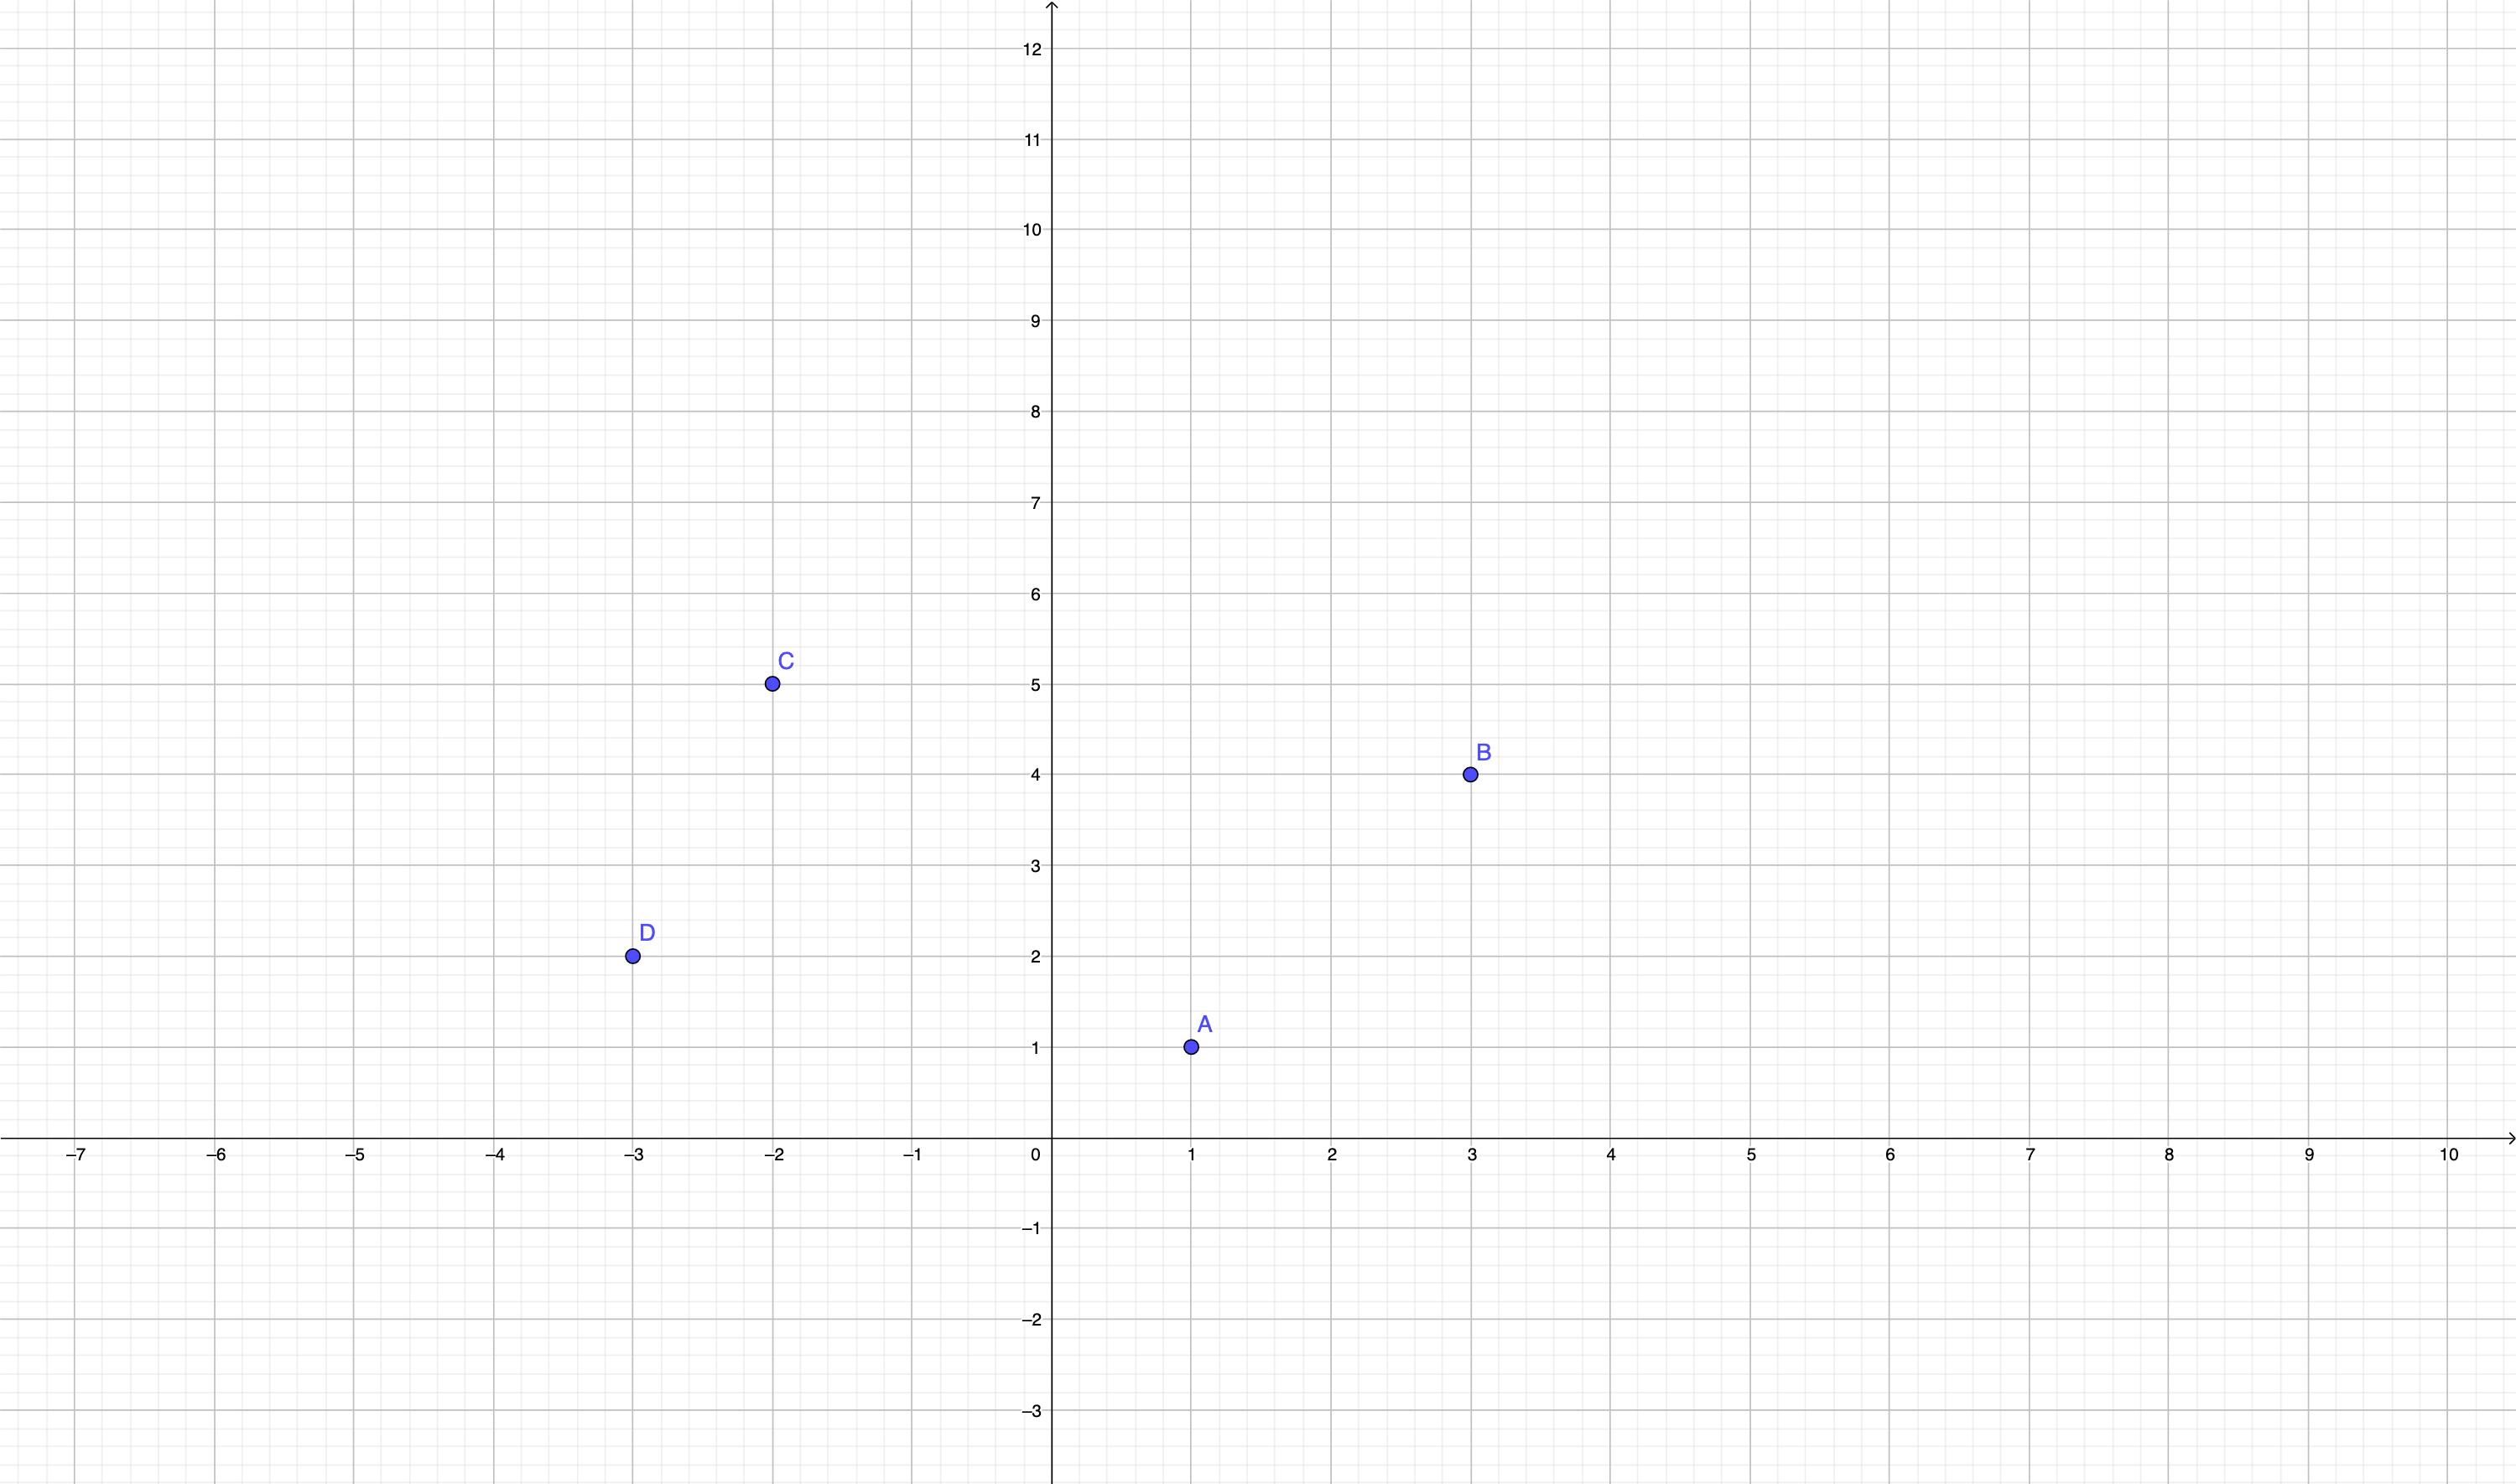
\includegraphics[scale=0.8]{Images/P1-1}
		\end{figure}
	\end{sol}
	\item Una de los puntos para obtener el cuadrilátero $ABCD$. 
		\begin{sol}
		.
		\begin{figure}[H]
			\centering
			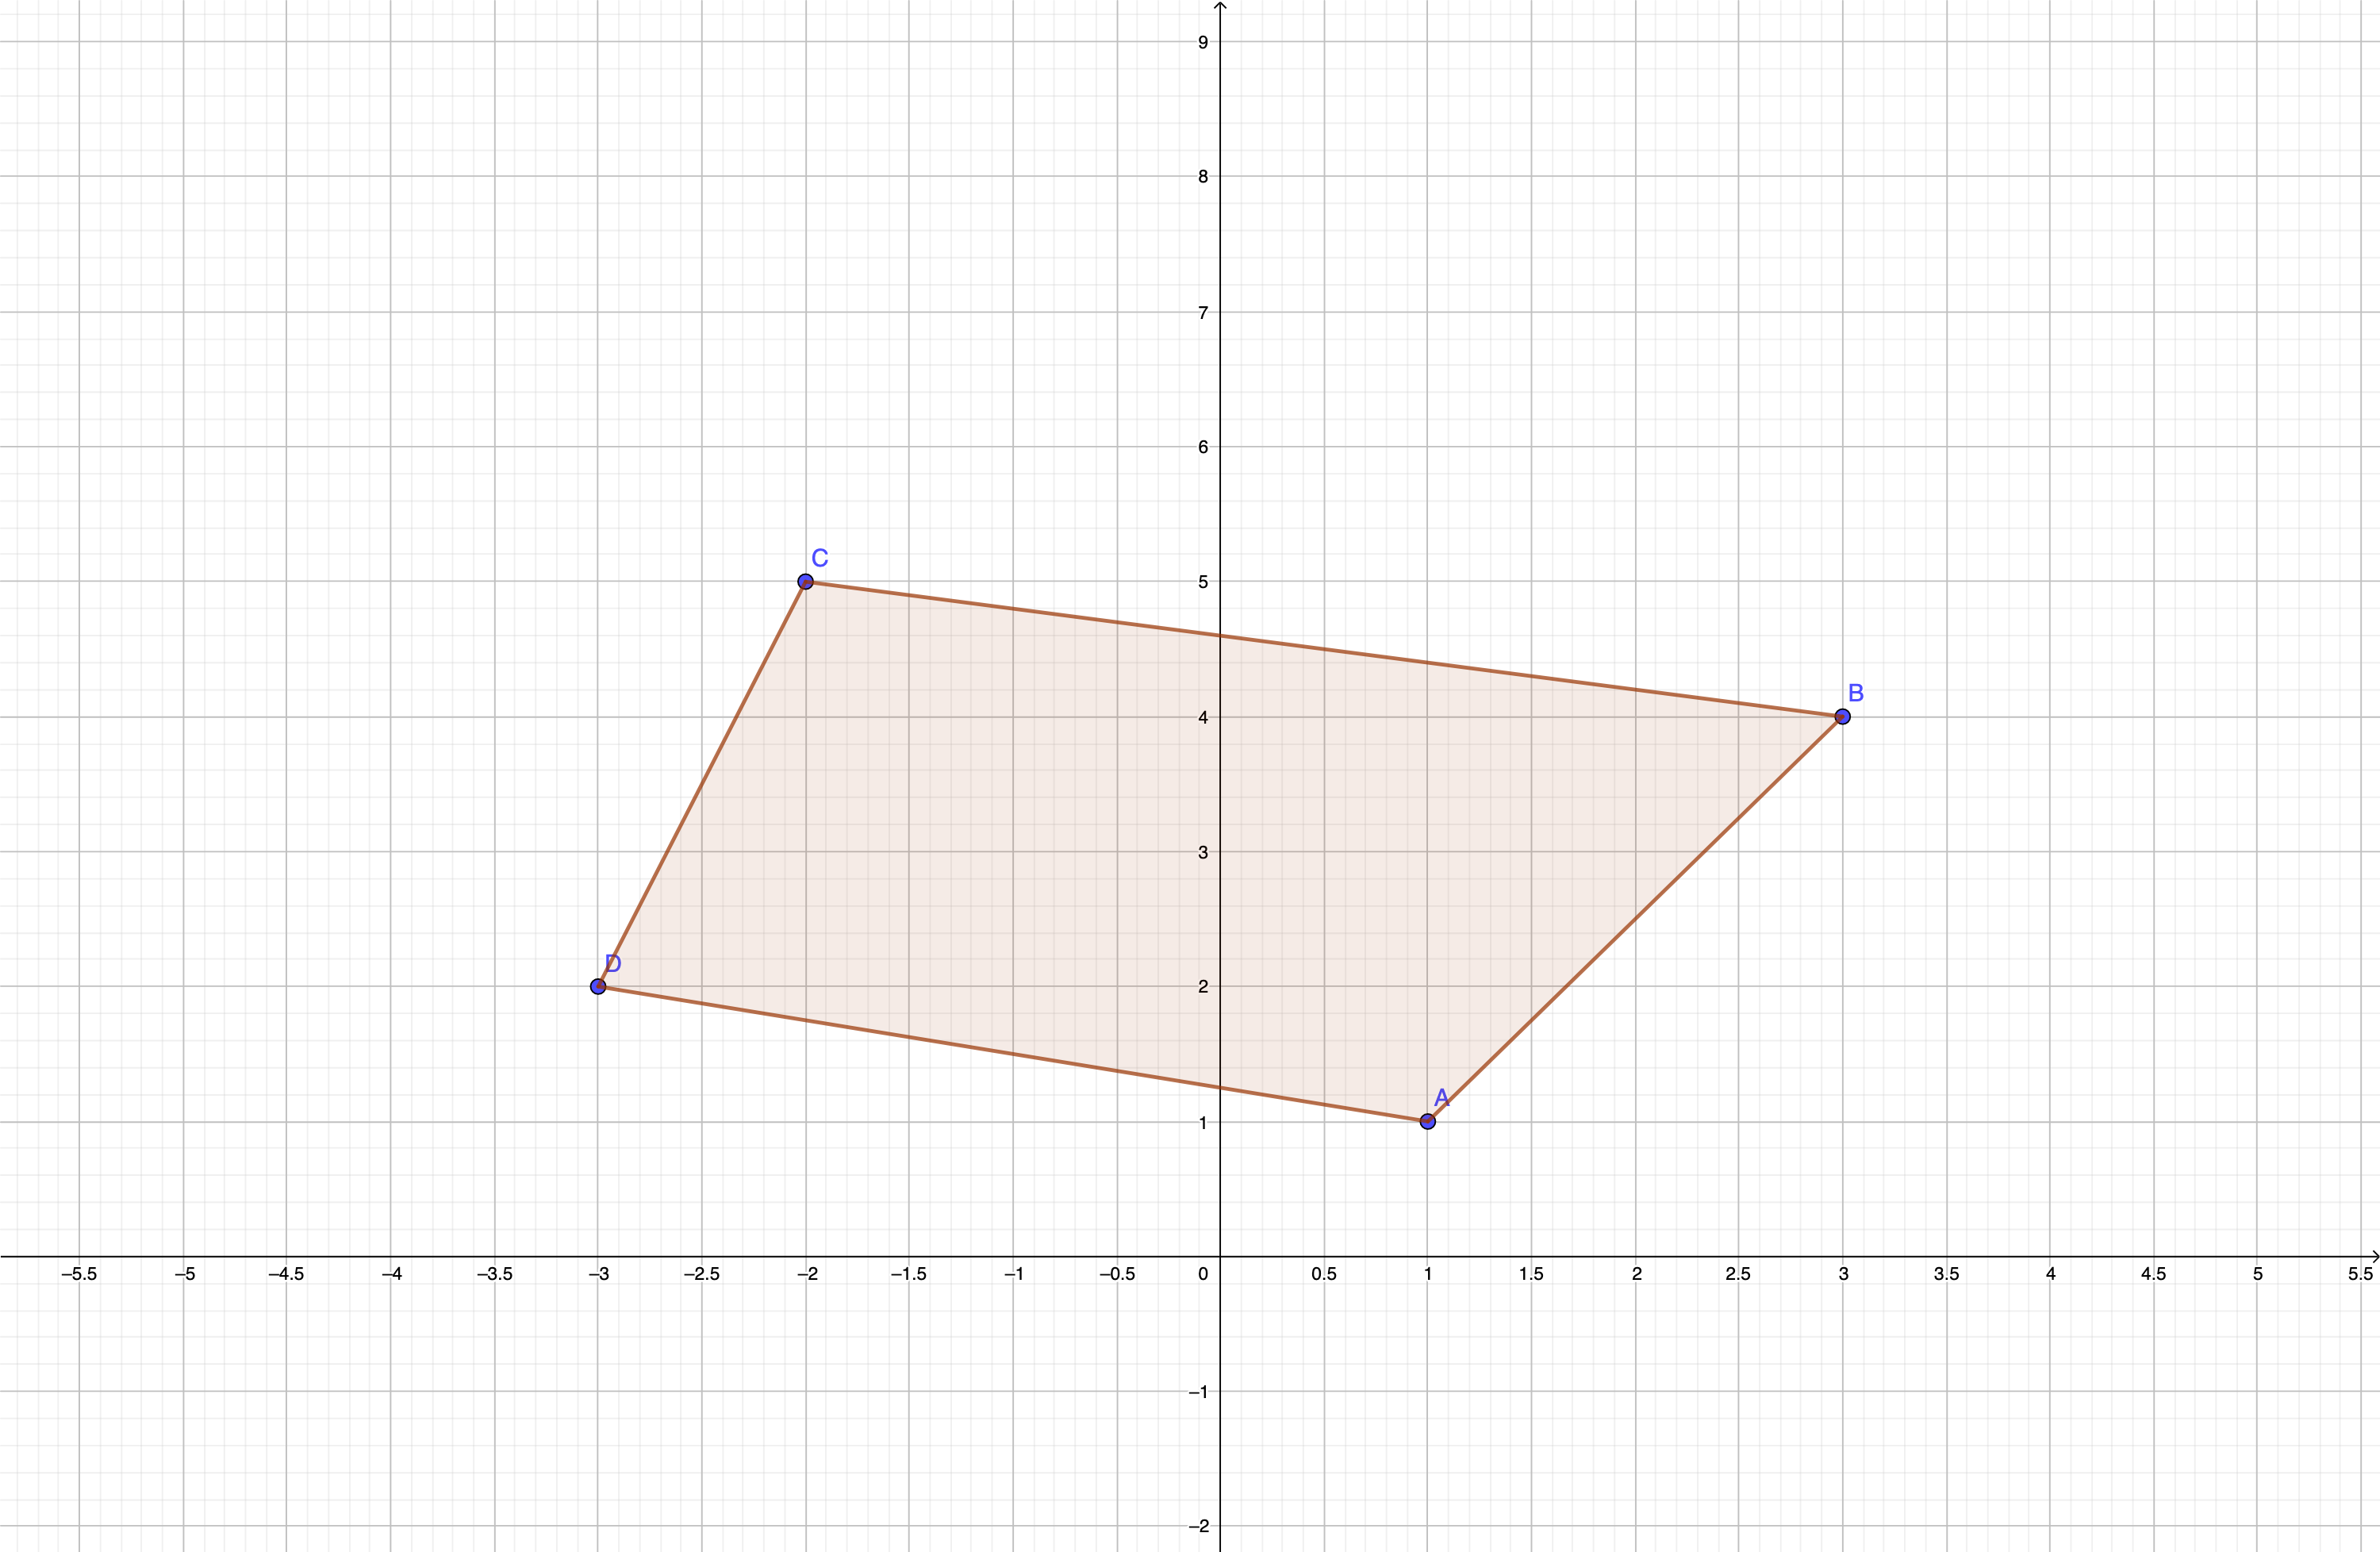
\includegraphics[scale=1]{Images/P1-2}
		\end{figure}
	\end{sol}
	\item Aplique ahora las siguientes transformaciones al cuadrilátero original: 
	\begin{enumerate}
		\item Una traslación en dirección del vector $0A$. 
		\begin{sol}
			$\overrightarrow{0A}$ consiste en una traslación (1,1), entonces a cada punto se le suman una unidad: $A(1+1,1+1)=A'(2,2)$, $B(3+1,4+1)=B'(4,5)$, $C(-2+1,5+1)=C'(-1,6)$ y $D(-3+1,2+1)=D'(-2,3)$. 
			\begin{figure}[H]
				\centering
				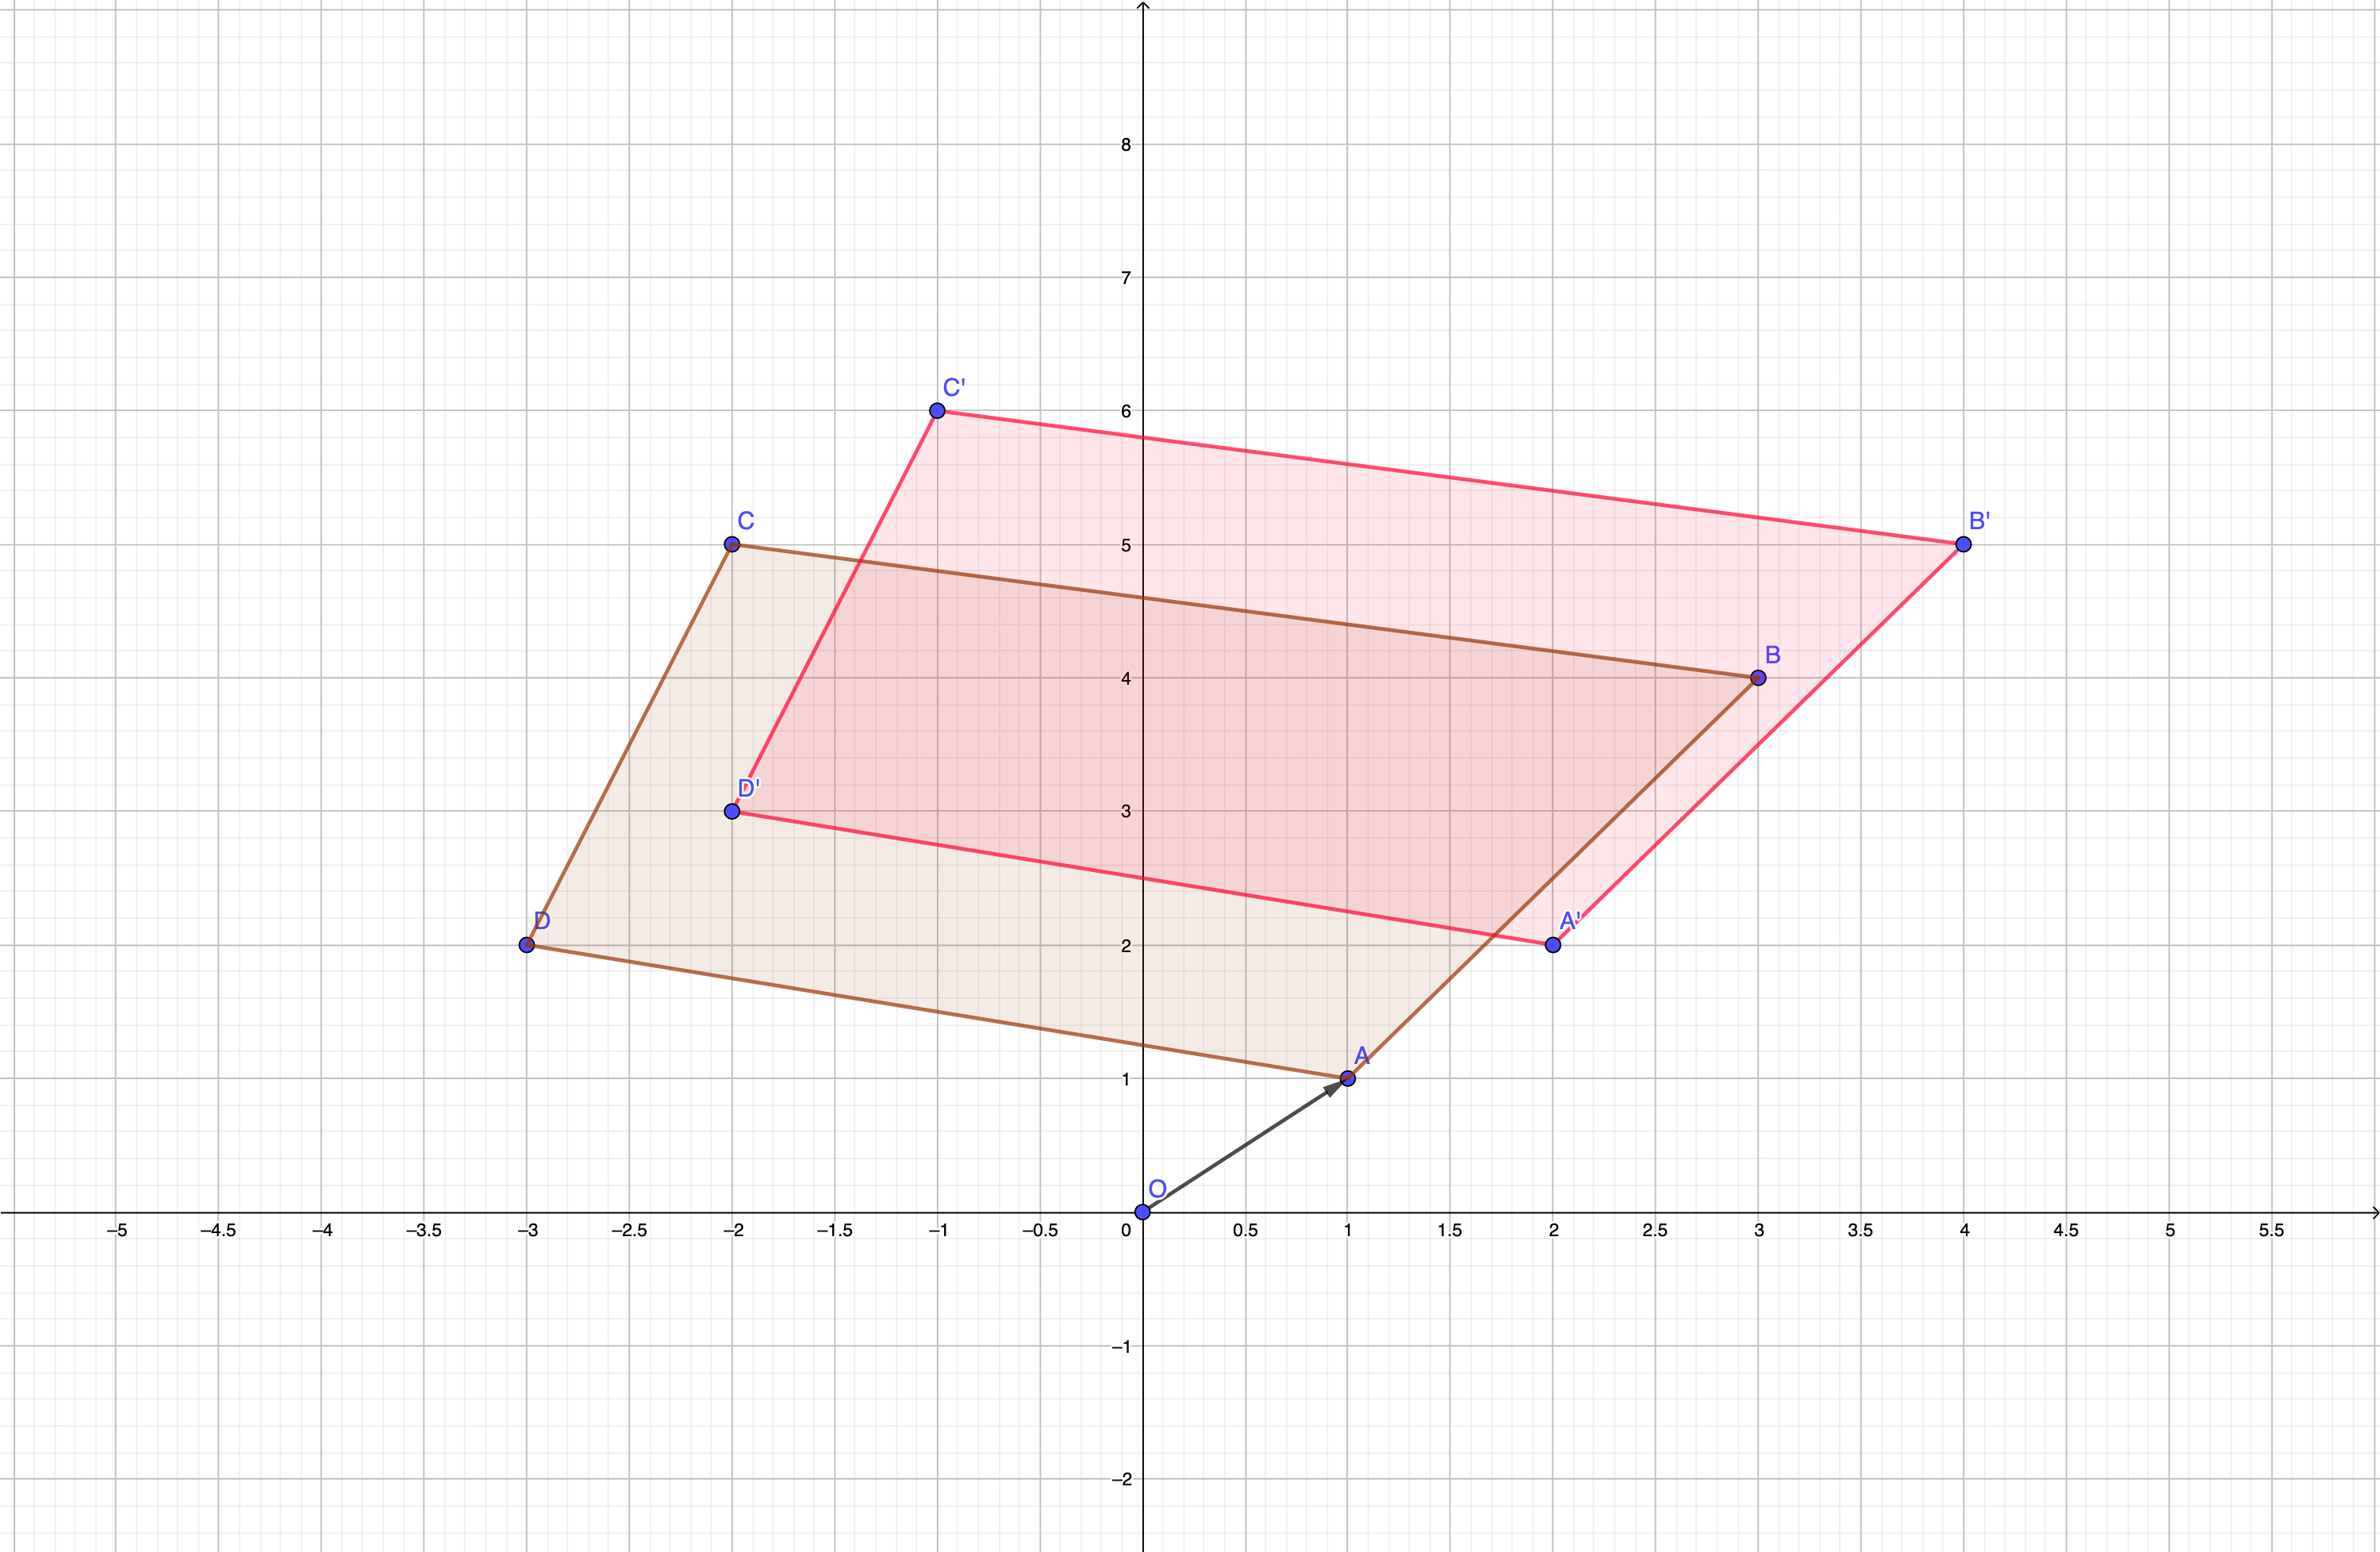
\includegraphics[scale=1]{Images/P1-3}
			\end{figure}
		\end{sol}
		\item Reflexión respecto al punto $E(-2,2)$. 
		\begin{sol}
			La ecuación para encontrar la reflexión dado un punto se define como: 
			$$\begin{cases}
				x' =2x_c-x\\
				y' =2y_c-y
			\end{cases}\implies\begin{cases}
			x' =2(-2)-x=-4-x\\
			y' =2(2)-y=4-y
		\end{cases} $$
	Por lo tanto, la nueva figura es: 
	$$A'(-5,3), B'(-7,0), C(-2,-1), D(-1,2).$$
			\begin{figure}[H]
				\centering
				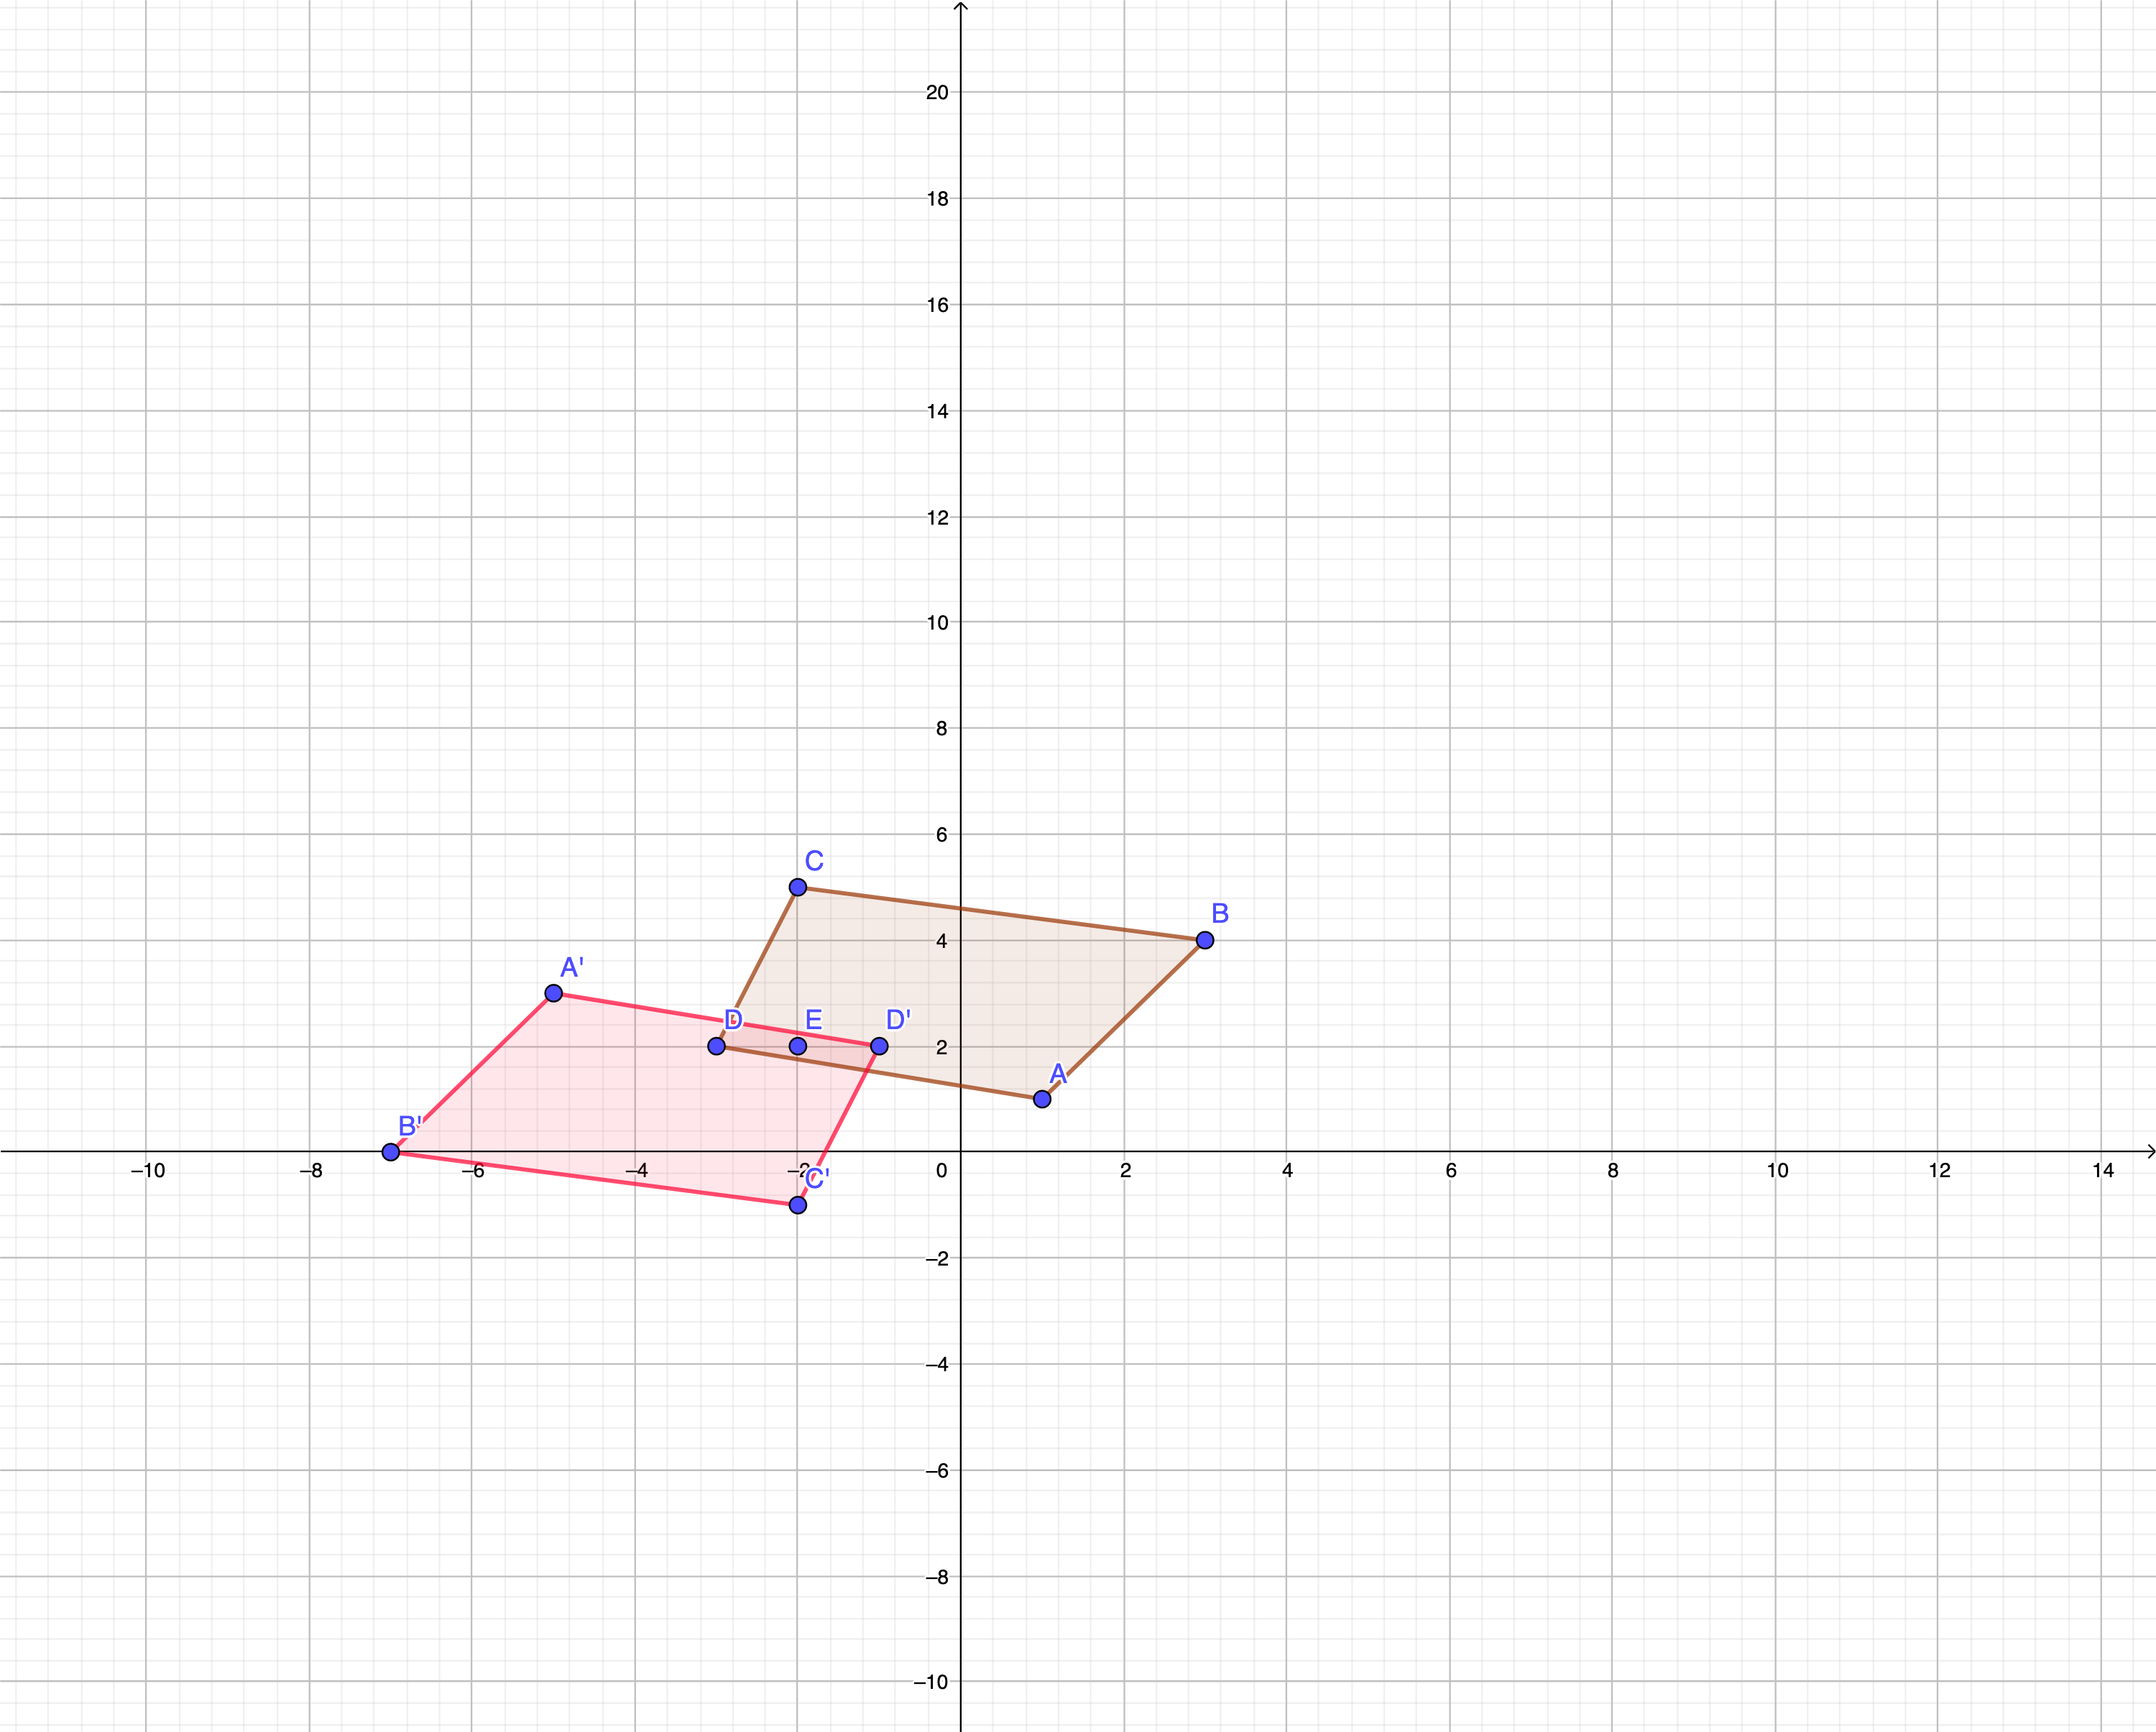
\includegraphics[scale=0.4]{Images/P1-c}
			\end{figure}
		\end{sol}
		\item Homotecia respecto al origen $(0,0)$ de $k=-(0.5)$. 
		\begin{sol}
			Usuaremos la ecuación siguiente para hacer la hometecia: 
			$$H(x,y)=\left(k(x-a)+a, k(y-b)+b\right), \quad k=factor, (a,b)=punto.$$
			Por lo que tenemos: 
			\begin{align*}
				H(x,y)&=\left(-0.5(x), -0.5(y)\right)\\
				A'(1,1)&=\left(-0.5(1), -0.5(1)\right)=(-1/2,-1/2)\\
				B'(3,4)&=\left(-0.5(3), -0.5(4)\right)=(-3/2,-2)\\
				C'(-2,5)&=\left(-0.5(-2), -0.5(5)\right)=(1,-5/2)\\
				D'(-3,2)&=\left(-0.5(-3), -0.5(2)\right)=(3/2,-1)			\end{align*}
			\begin{figure}[H]
				\centering
				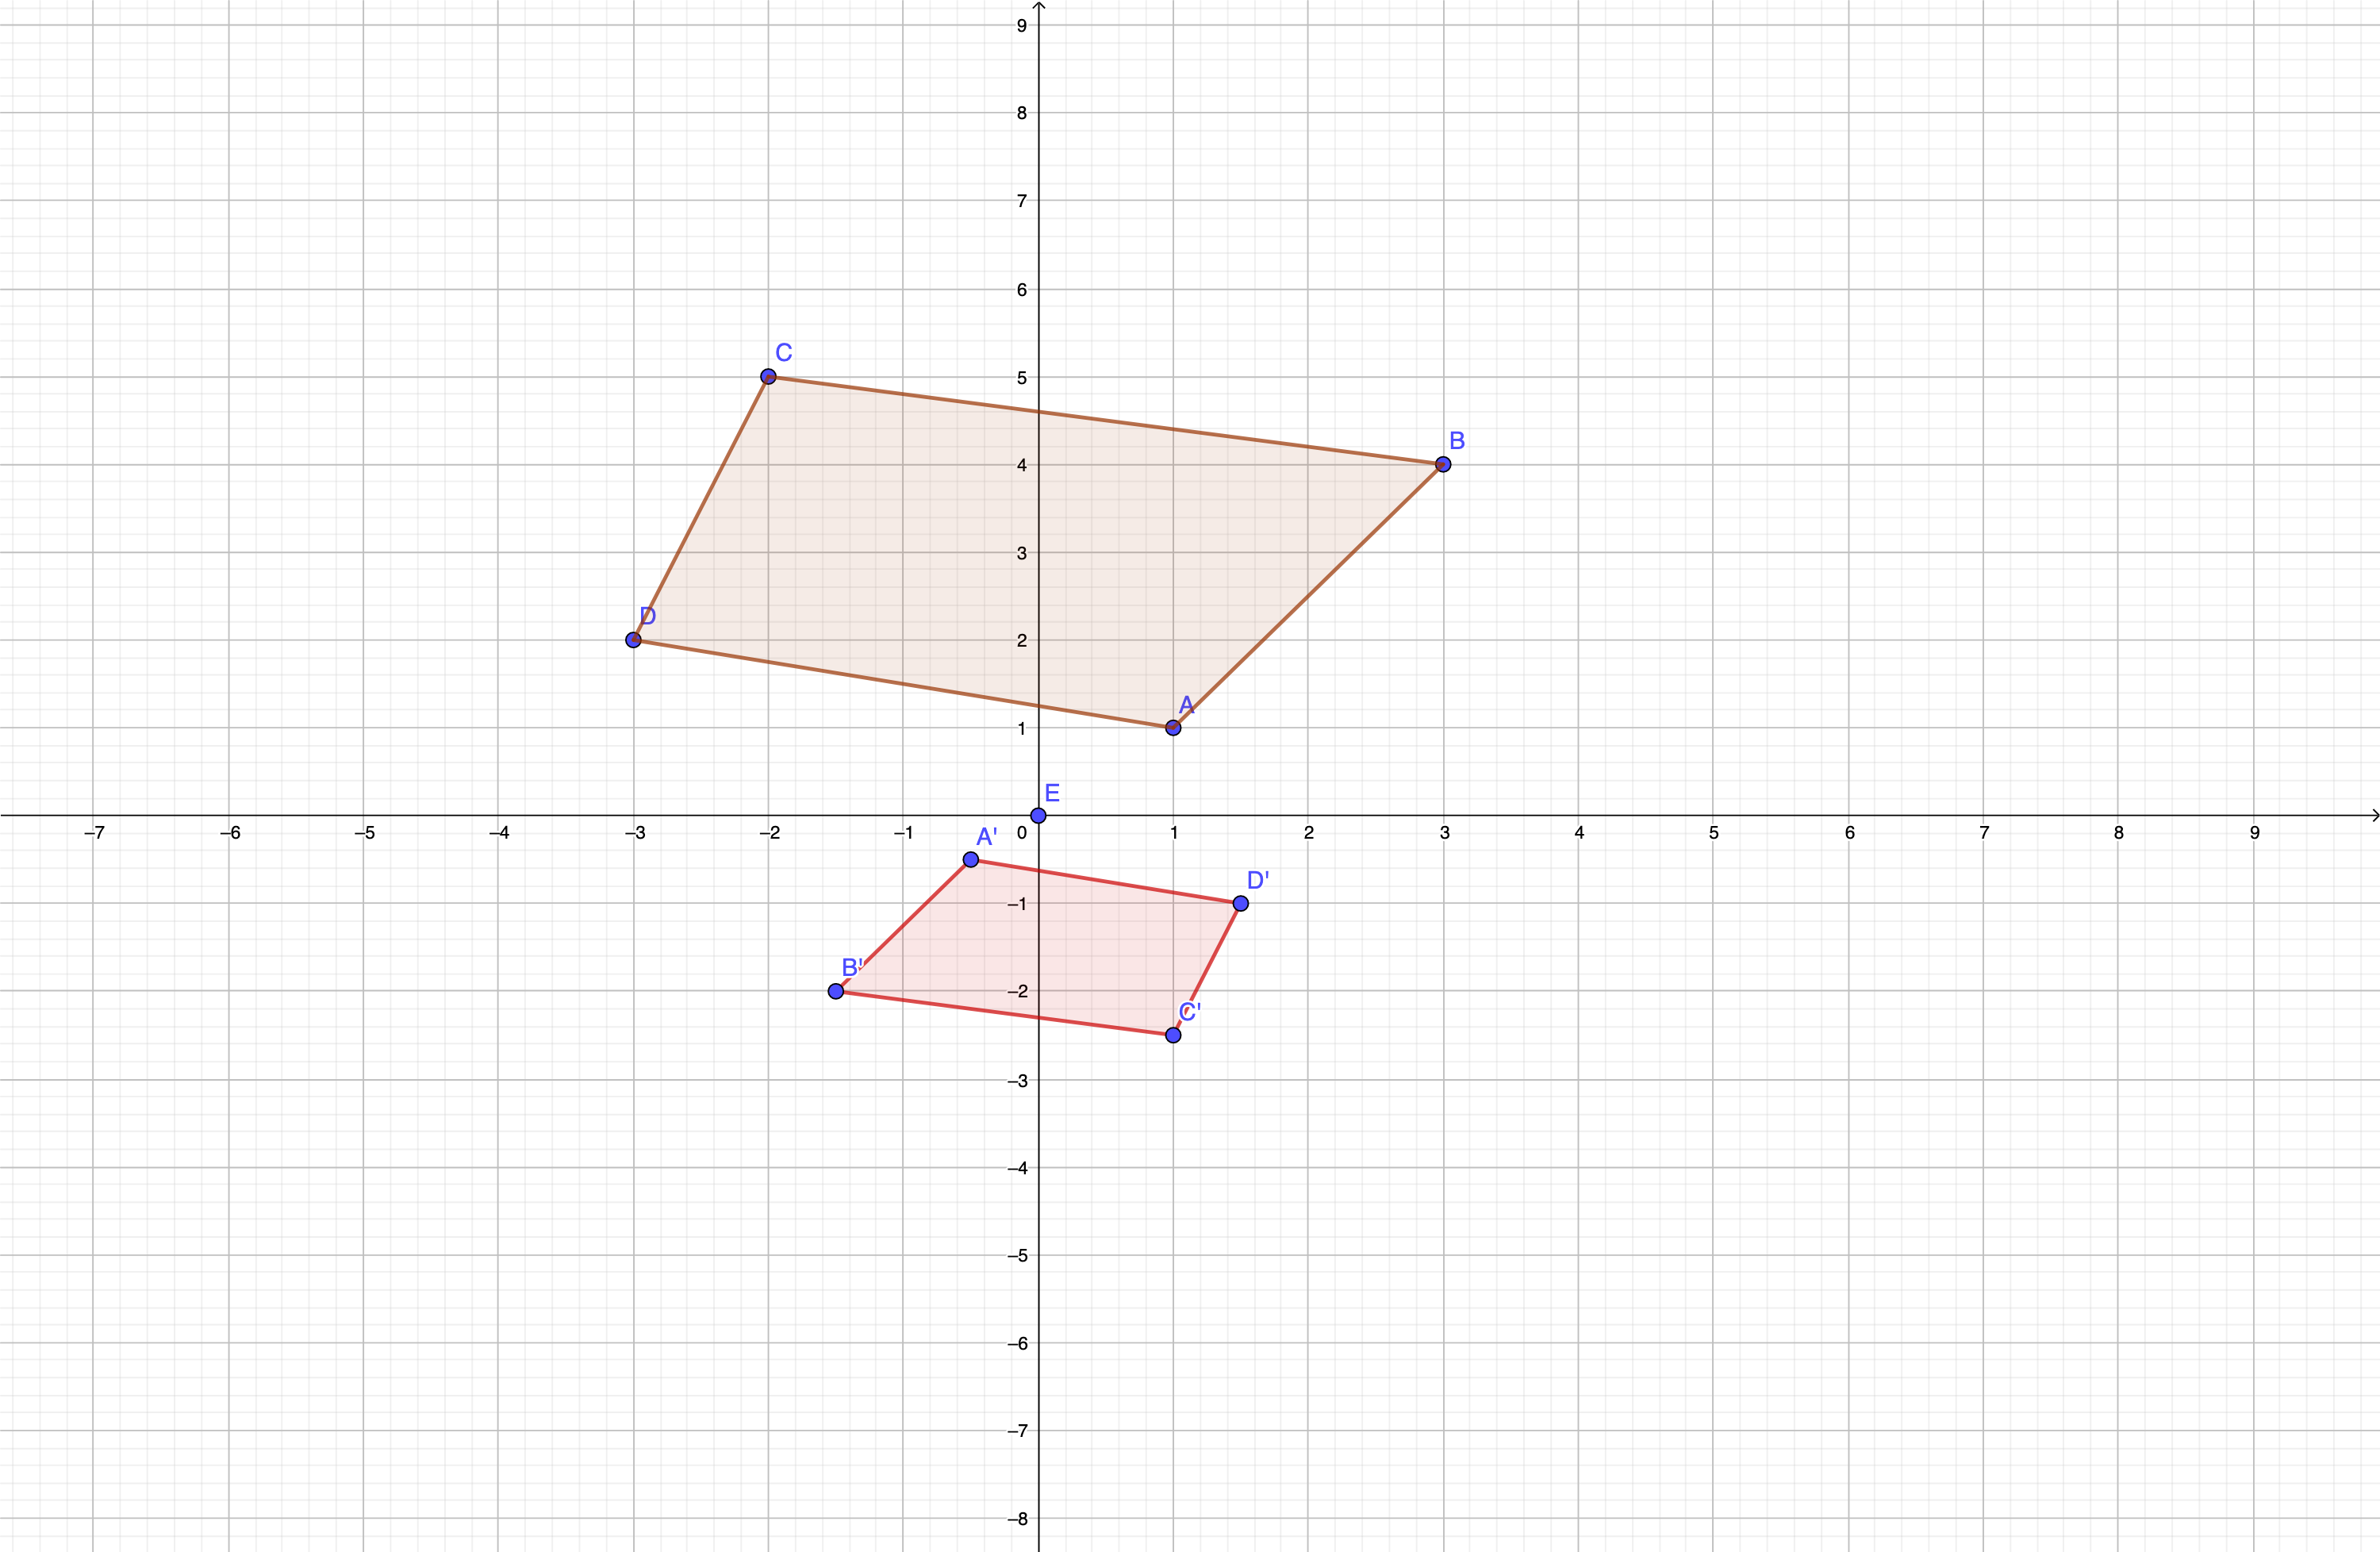
\includegraphics[scale=0.7]{Images/P1-5}
			\end{figure}
		\end{sol}
	\end{enumerate}
\end{enumerate}
\end{problema}